\documentclass[11pt,a4paper]{article}
\usepackage[T1]{fontenc}
\usepackage[utf8]{inputenc}
\usepackage[margin=2.5cm]{geometry}
\usepackage{graphicx,booktabs,array,hyperref,float}
\usepackage[table]{xcolor}
\setlength{\parindent}{0pt}
\setlength{\parskip}{5pt}
\hypersetup{colorlinks=true,urlcolor=blue}
\title{\vspace{-1.2cm}Physical climate risk screening of an infrastructure portfolio:\\ flood and heat, adaptation finance tagging and a simplified Paris-alignment check\vspace{-0.3cm}}
\author{Mikhail Serikov \\ \small Research study on open data, Belgrade case, November 2026}
\date{}
\begin{document}
\maketitle

\section*{1. Purpose and case}
This note shows how a project portfolio can be screened for physical climate risk with public data, how adaptation measures are chosen when the climate scenario is uncertain, and how the measures are tagged as adaptation finance and checked for alignment. The case is a set of 331 water, energy, transport and hospital assets around Belgrade, Serbia, taken from OpenStreetMap. Asset values, damage curves, measure costs and scenario factors are assumptions listed in the repository (\texttt{data/sources.csv}). The results show the method and orders of magnitude; they are not a valuation of real assets and not the methodology of any institution.

\section*{2. Method in six steps}
\begin{enumerate}
\setlength\itemsep{1pt}
\item \textbf{Exposure.} Flood depth at each asset from the JRC / CEMS GloFAS river flood hazard maps (3 arc seconds, return periods 10, 50, 100, 200 and 500 years). Of the 331 assets, 23 sit in or on the bank of a river channel that the 90 m grid cannot resolve (1-in-10 depth of at least 2 m); they are excluded from the totals and listed for site review. 308 assets with an assumed value of 2,460 million EUR remain.
\item \textbf{Expected annual loss.} Depth-damage curve per asset class times assumed value, integrated over exceedance probability. Damage from floods more frequent than the 1-in-10 flood is set to zero, so the flood loss is a lower bound.
\item \textbf{Heat.} Days above 35~\textdegree C from ERA5 daily maxima 1991--2020 at the grid point near Belgrade, shifted by the change of three CMIP6 models between 1995--2014 and 2041--2060 per quantile of daily maximum temperature (quantile delta method), times an assumed loss rate per day.
\item \textbf{Scenarios.} Baseline, moderate (flood frequency $\times$1.3, heat of SSP2-4.5) and high ($\times$2.0, heat of SSP5-8.5; median of three models). The flood factors are stress factors, not projections.
\item \textbf{Measures.} A local barrier (0.5 m), a flood wall (1.5 m) and elevation of critical equipment (3 m), with cost shares of asset value, annualised at 6\% over 30 years. The plan is chosen per scenario and by minimax regret across scenarios; the value of knowing the scenario (EVPI) is computed.
\item \textbf{Tagging and alignment.} Each chosen measure is tagged by a three-step rule (vulnerability, intent, direct link) and each asset is screened against a simplified alignment rule.
\end{enumerate}

\section*{3. Findings}
\begin{table}[H]
\centering\small
\begin{tabular}{lrrr}
\toprule
 & Baseline & Moderate & High\\
\midrule
Expected annual flood loss, million EUR & 4.7 & 6.1 & 9.4\\
Days per year above 35~\textdegree C & 8.3 & 23.8 & 28.5\\
Expected annual heat loss (assumed rate), million EUR & 4.4 & 12.6 & 15.1\\
Net benefit of the minimax-regret plan, million EUR/yr & 3.05 & 4.34 & 7.35\\
\bottomrule
\end{tabular}
\end{table}
Only 18 of the 308 assets have a 1-in-100 flood depth of at least 0.1 m. Transmission substations carry 48\% of the baseline flood loss, water works 20\% and pumping stations 16\%. The flood loss doubles in the high scenario and the heat loss more than triples, so the heat loss matters as much as the flood loss, although its rate is an assumption.

\begin{figure}[H]
\centering
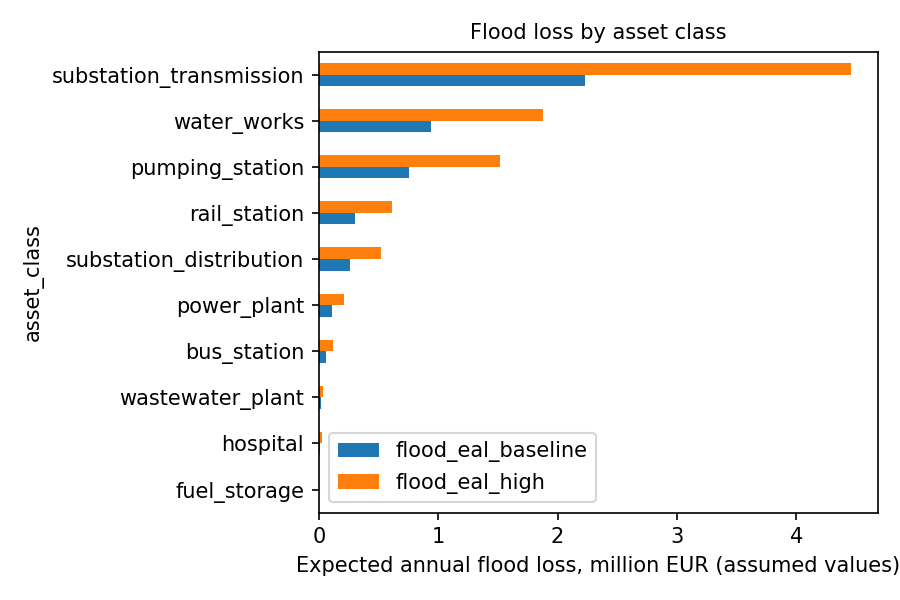
\includegraphics[width=0.48\textwidth]{../results/fig_flood_eal_by_class.png}\hfill
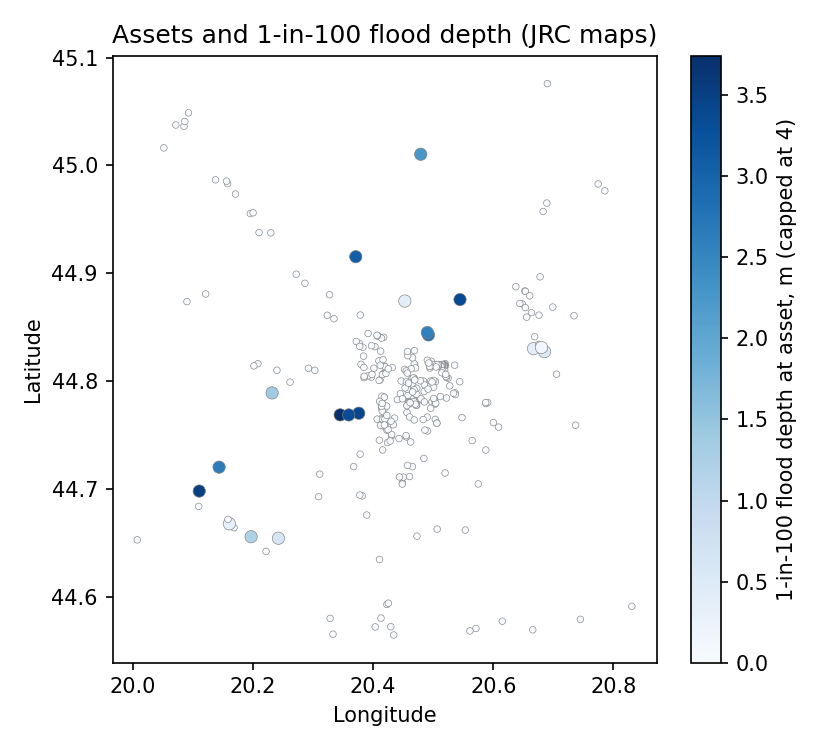
\includegraphics[width=0.48\textwidth]{../results/fig_asset_map.png}
\caption{Left: expected annual flood loss by asset class, baseline and high scenario (assumed values). Right: assets and the 1-in-100 flood depth from the JRC maps.}
\end{figure}

The minimax-regret plan puts a measure on 17 assets (10 equipment elevations, 5 flood walls, 2 local barriers) at a capital cost of 15.1 million EUR. Its maximum regret over the three scenarios is 0.026 million EUR per year, against 0.101 for the plan optimised for the baseline and 0.049 for the plan optimised for the high scenario. The value of knowing the scenario is 0.010 million EUR per year, about 0.3\% of the baseline net benefit. For these assets the choice of measure does not depend on resolving the scenario; the size of the loss does.

\begin{figure}[H]
\centering
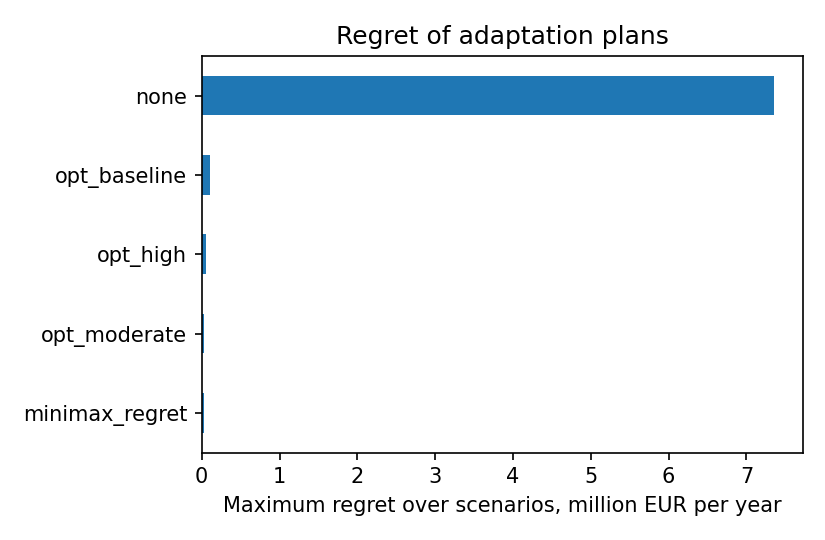
\includegraphics[width=0.62\textwidth]{../results/fig_plan_regret.png}
\caption{Maximum regret of the plans over the three scenarios.}
\end{figure}

\section*{4. Adaptation finance tagging and alignment}
The tagging rule follows the three-step structure of the MDB-IDFC common principles for climate finance tracking: a context-specific vulnerability (1-in-100 depth of at least 0.1 m or 1-in-500 depth of at least 0.5 m), an explicit intent to reduce it, and a direct link (the measure height at least equal to the 1-in-100 depth). Eleven of the 17 measures pass all three steps, which tags 10.7 of the 15.1 million EUR. Six measures are not tagged as stated because the height is below the 1-in-100 depth, so the link to the vulnerability is only partial; confirming a higher design would move them into the tagged amount. Every decision is stored with its numbers in \texttt{results/tagging\_and\_paris\_screen.csv}.

The simplified alignment screen has four outcomes. 284 assets are aligned because the physical flood risk is not material (below 0.05\% of value per year). Five are aligned if the measure is part of the project scope. Twelve are not yet aligned because the selected measure leaves the residual loss above the threshold. Seven are not aligned: the risk is material and none of the three measures pays for itself. The rule is a screening device in the structure of the MDB joint approach and not the methodology of any institution.

\section*{5. Policy options}
\begin{enumerate}
\setlength\itemsep{2pt}
\item \textbf{Screen at asset level at project entry.} Eighteen of 308 assets hold nearly all of the flood loss, so a country or sector flag would miss where the risk is. A fixed rule (exposure at the 1-in-100 and 1-in-500 depth from an open hazard map) is cheap and traceable.
\item \textbf{Set a design standard that matches the tagging rule.} Requiring protection at least to the 1-in-100 depth turns the six partly linked measures into fully tagged adaptation finance and avoids undersized designs.
\item \textbf{Use scenario-robust selection.} Choosing by minimax regret over at least two scenarios lowers the maximum regret to 0.026 from 0.101 million EUR per year without needing a scenario forecast. The flood loss rises linearly with the frequency factor (14.1 million EUR at $\times$3), so the stress range should be stated in the project file.
\item \textbf{Offer other instruments where hard protection does not pay.} For the seven assets that are not aligned, options are operating rules, relocation of critical equipment, contingency funding or insurance, and a closer look at whether the asset is needed at its location.
\item \textbf{Fund the data step.} Twenty-three assets could not be screened with a 90 m map. Local survey data or a finer hazard model for such sites is a candidate for technical cooperation funding, and the screening code can be shared with clients so that they can repeat it.
\end{enumerate}

\section*{6. Limits}
Values, damage curves, measure costs, the heat loss rate and the scenario factors are assumptions. The flood maps are riverine only, for the historical climate, with known artefacts in channels; a 3\,$\times$\,3 pixel window maximum doubles the portfolio loss (9.1 against 4.7 million EUR), which shows the sensitivity to position error. The asset set is an OpenStreetMap sample, not an inventory. The heat scenarios use three CMIP6 models (one member each, 20-year windows, one grid cell near Belgrade), so the models differ by up to 10 days a year and the median is not a projection. Code, data manifest and tests: \url{https://github.com/serikov-climate-risk/climate-risk-screening}.
\end{document}
